
\section{enzymes.xml}

\subsection{Rationale}

The enzyme file is used to define enzyme composition and their catalytic efficiency.
It defines efficiency constraints in the RBA model.
These constraints ensure that a reaction flux is smaller than
the product of efficiency and concentration of the enzyme catalyzing
the reaction.

So far, we have defined two types of basic molecules:
metabolites (in metabolism.xml) and macromolecules (e.g.\ in proteins.xml).
There is a third type of molecule in RBA models called a \emph{molecular machine}.

Molecular machines are composed of metabolites and macromolecules.
Contrary to macromolecules, who share a small pool of components and undergo
complex assembly processes, molecular machines can be composed of any
metabolite or macromolecule, and their assembly is described by a single reaction.
Molecular machines also have a functional role within the cell:
catalyzing metabolic reactions or assisting the assembly of macromolecules.

Enzymes are the simplest molecular machines in RBA models,
their role is to catalyze metabolic reactions (as defined in metabolism.xml).
Process machines are the other molecular machines in RBA models,
their composition is defined identically to enzymes,
but characterizing their role in the assembly of macromolecules,
although similar to the catalysis description, is significantly more complex
(as we will see in processes.xml).

The definition of enzymes contains three parts:
the composition of the enzyme, the reaction the enzyme catalyzes,
and the forward and backward efficiencies of the enzyme.
Only one enzyme can be associated with a reaction:
if a reaction may be catalyzed by several enzyme,
it must be duplicated so that every enzyme can be associated with a separate
reaction.

\subsection{RBAEnzymes}
\label{sec:rba_enzymes}

The outermost part of the metabolism file is an instance of class
\rbaenzymes, shown in Figure~\ref{fig:enzymes_doc}.

\begin{figure}
  \centering
  \includegraphics[scale=0.8]{figures/enzymes_doc}
  \caption{XML structure of enzyme document.}
\label{fig:enzymes_doc}
\end{figure}

\rbaenzymes{} has no simple attributes.
It contains excatly one instance of \textbf{ListOfEnzymes} that is used
to store \enzyme{} information.


\subsection{Enzyme}
\label{sec:enzyme}

The \enzyme{} class is used to define enzymes
(Fig.~\ref{fig:enzymes_doc}).

It contains a \machinerycomposition{} that refers to metabolic \species{}
and \macromolecule{}s composing the \enzyme{}.
Note that the composition can be left unspecified.
In this case, the reaction associated with the enzyme is considered spontaneous.

\paragraph{The \textit{id} attribute}
The \textbf{id} attribute is a string defining the identifier of
the enzyme.

\paragraph{The \textit{reaction} attribute}
The \textbf{reaction} attribute must match the identifier of a metabolic
\reaction.
It represents the reaction catalyzed by the enzyme.
This must be a one-to-one mapping.
A \reaction{} can only have one associated \enzyme{}.
If several \enzyme{}s catalyze the same \reaction{},
the \reaction{} must be duplicated.

\paragraph{The \textit{forwardEfficiency} attribute}
The \textbf{forwardEfficiency} attribute must match the identifier of a
parameter (\function{} or \aggregate{}).
It represents the forward catalytic constant.

\paragraph{The \textit{backwardEfficiency} attribute}
The \textbf{backwardEfficiency} attribute must match the identifier of a
parameter (\function{} or \aggregate{}).
It represents the backward catalytic constant
(only applicable if reaction catalyzed by enzyme is reversible).

\paragraph{The \textit{zeroCost} attribute}
The \textbf{zeroCost} attribute is a boolean value.
If set to true, the reaction associated may occur without having to produce
the enzyme.
If set to false or unspecified, an efficiency constraint is created where the
flux through the reaction has to be smaller than the product of enzyme
efficiency and enzyme concentration.

\subsection{Examples}

A typical enzymes.xml contains a long list of enzymes
(Fig.~\ref{fig:enzymes_ex_1}),
typically one enzyme per metabolic reaction (Fig.~\ref{fig:enzymes_ex_2}).
If a reaction occurs spontaneously, it is not technically necessary to
associate a reaction with it, but RBApy creates an enzyme none-the-less,
showing that the reaction was correctly identified as spontaneous.

The \machinerycomposition{} is identical to a metabolic reaction,
except that it may contain macromolecules, not just metabolites.
In the two examples, enzymes are composed of proteins, with identifiers
defined in proteins.xml.
The reaction could also have included byproducts by defining a \texttt{ListOfProducts}.
A typical example would have been the inclusion of GTP as a reactant and GDP
as a byproduct of the assembly of some enzymes, but we neglected these costs in our models.

Note that the efficiencies are \emph{not} numerical values:
they are parameter identifiers, all parameters of the model being defined in parameters.xml.
Also note that \texttt{zero\_cost} is a flag that is almost always set to false.
Setting it to true effectively removes the enzyme, making the associated reaction
spontaneous.
It was included for retrocompatibility with early RBA versions, where it was
used to counterbalance numerical instabilities.



\begin{figure}
  \centering
  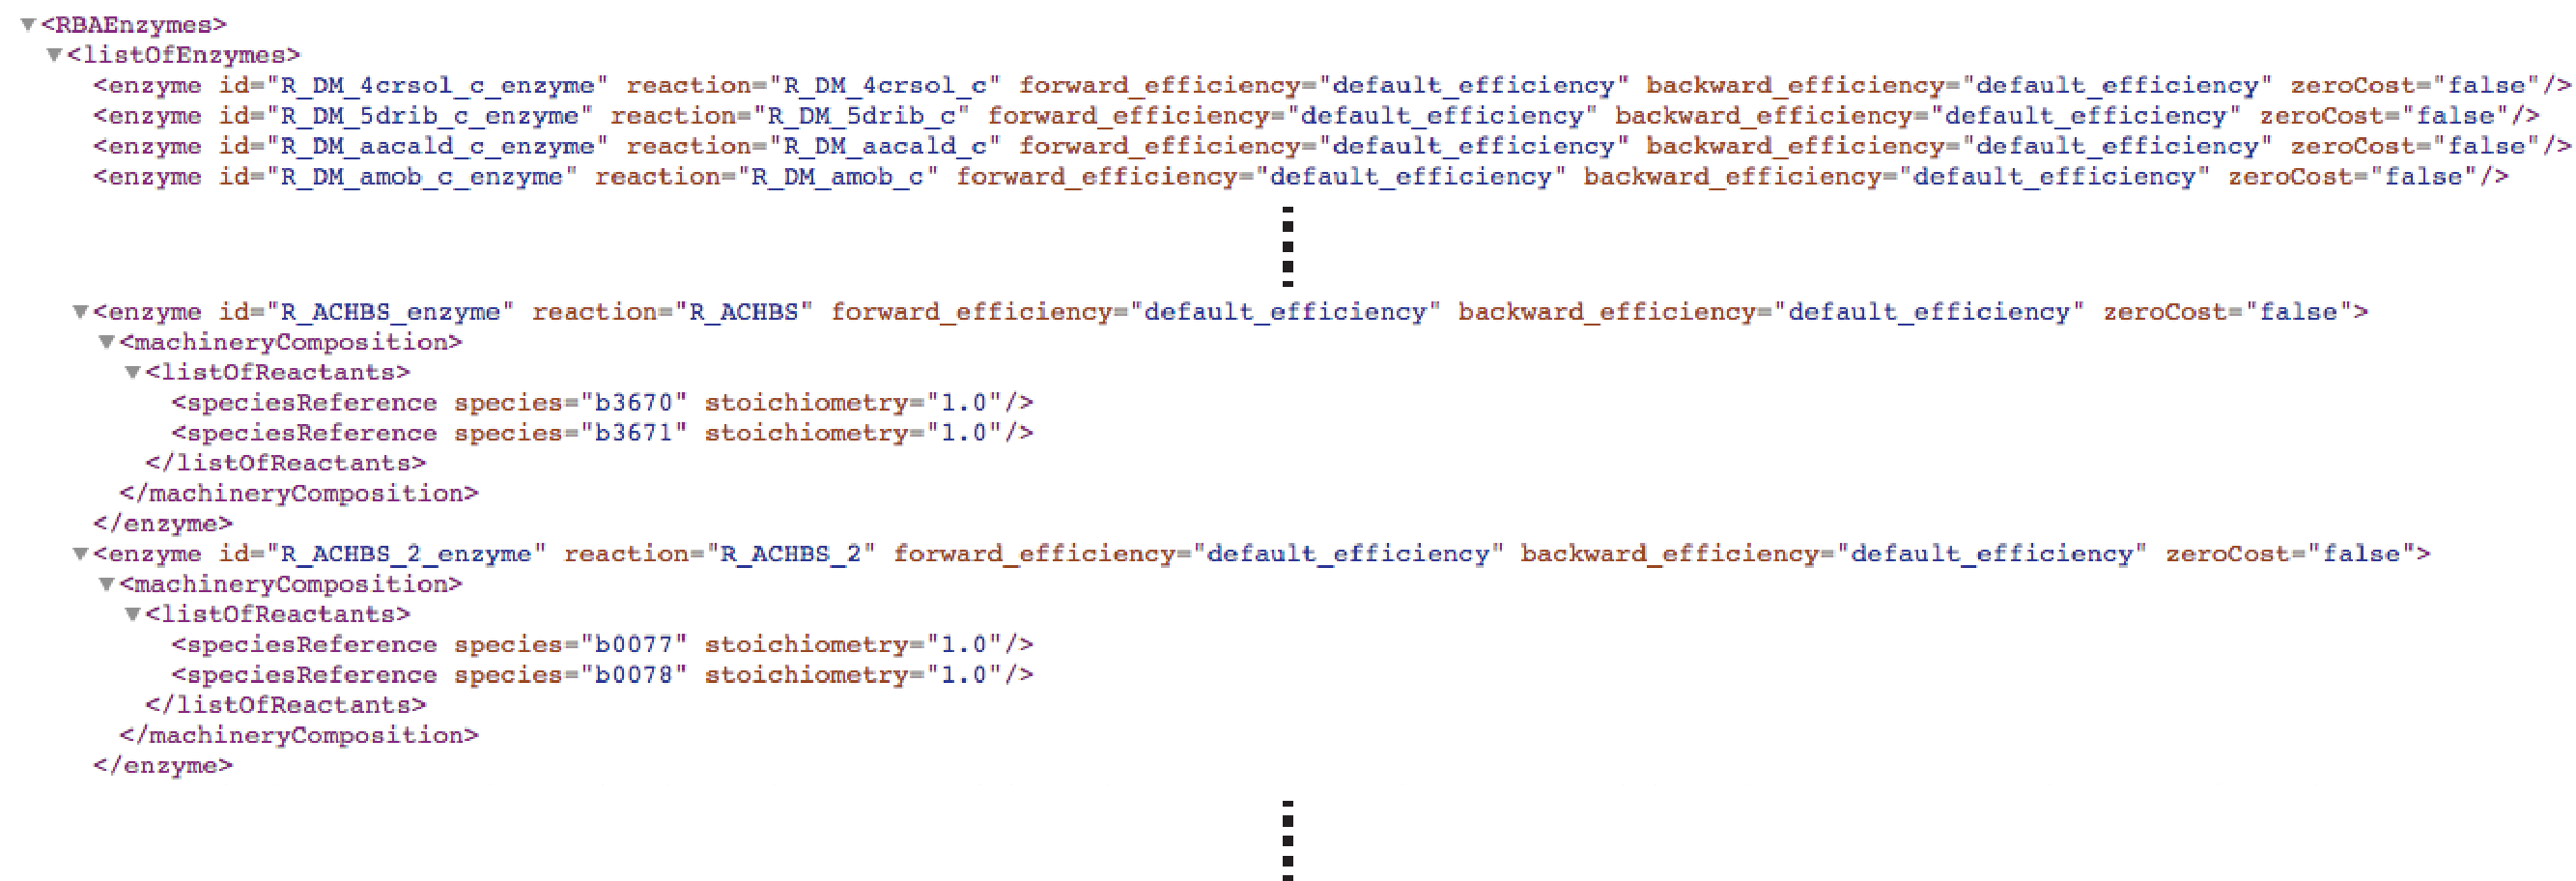
\includegraphics[scale=0.4]{figures/enzymes_ex_1}
  \caption{enzymes.xml from a model automatically generated by RBApy for the
  model bacteria \textit{E. coli}.
  Large chunks of the files were removed for brevity.
  The list starts with 4 enzymes with no composition, indicating that
  the associated reactions occur spontaneously.
  The last two enzymes have different compositions but are associated with
  identical metabolic reactions:
  either of these enzyme may be produced by the cell to catalyze the reaction.}
  \label{fig:enzymes_ex_1}
\end{figure}

\begin{figure}
  \centering
  \includegraphics[scale=0.4]{figures/enzymes_ex_2}
  \caption{enzymes.xml from the minimal model.
  We associate one enzyme with all 3 reactions defined in metabolism.xml.
  Enzymes are defined by using the proteins that we defined in proteins.xml.}
  \label{fig:enzymes_ex_2}
\end{figure}
